\chapter{Methods}
\begin{itemize}
\item Introduce requirements
\item Need to preserve spatial information for symbolic front-end
\item Need disentangled latent space for symbolic front-end
\item Explain degree of freedom here (disentangled filters, or disentangled neurons, or something else?)
\item This is unexplored territory here - we decide what the reasonable architecture should be
\end{itemize}

\label{ch:methods}


%
%
%
%
%
\section{Dimensionality Reduction}

Machine learning with high-dimensional data, such as images, is often computationally intensive. Atari frames are RGB images ($3$ channels) of size $210 \times 160$, expressed in shorthand as $(3, 210, 160)$. (This data is much higher in dimensionality than MNIST, which has dimensions $(1, 28, 28)$). Considering the training sets considered in this project are of hundreds of thousands of images, data points of dimension $(3, 210, 160)$ are too computationally intensive with the best hardware available (2 $\times$ NVIDIA Tesla K80 GPU Accelerator). It is therefore necessary to reduce the dimensionality of our data set. Google DeepMind's \textit{Human-level Control Through Deep Reinforcement Learning} \cite{Mnih2015} made use of Stella, as we have, and have convincingly struck a reasonable balance between resolution and dimensionality reduction. This section will be a short but necessary mentioning of the preprocessing pipeline used to generate the data sets in later chapters.


\subsection{Pre-processing Stella Frames}

\subsubsection{Sprite Rendering in Stella}
Stella generates Atari frames of size $210 \times 160$ with a 128 colour palette. Atari 2600 games can only store a limited number of sprites per frame due to the limitations in hardware during its development \cite{Mnih2015}. This is an issue as some objects that appear in one frame fail to appear in the next. To solve this lack of object persistence, even and odd frames are combined by taking the maximum over each channel (RGB). By taking the maximum, we ensure that any object present in one frame is also present in the other. 

\begin{figure*}
\centering
\captionsetup{justification=centering}
\begin{multicols}{3}
    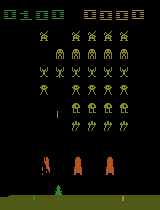
\includegraphics[scale=0.8]{figures/related_work/space_invaders_341_rgb_even.png}\par 
    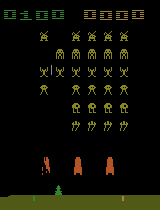
\includegraphics[scale=0.8]{figures/related_work/space_invaders_341_rgb_odd.png}\par
    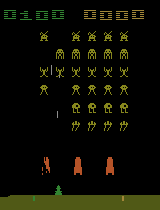
\includegraphics[scale=0.8]{figures/related_work/space_invaders_341_rgb_maximum_of_even_odd.png}\par    
    \end{multicols}
\begin{multicols}{3}
    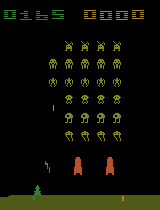
\includegraphics[scale=0.8]{figures/related_work/space_invaders_831_rgb_even.png}\par
    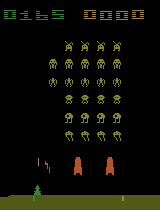
\includegraphics[scale=0.8]{figures/related_work/space_invaders_831_rgb_odd.png}\par
    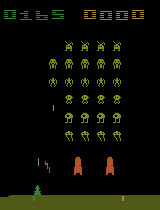
\includegraphics[scale=0.8]{figures/related_work/space_invaders_831_rgb_maximum_of_even_odd.png}\par
\end{multicols}
\begin{multicols}{3}
    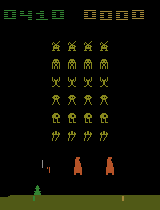
\includegraphics[scale=0.8]{figures/related_work/space_invaders_1044_rgb_even.png}\par
    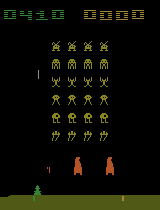
\includegraphics[scale=0.8]{figures/related_work/space_invaders_1044_rgb_odd.png}\par
    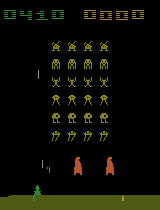
\includegraphics[scale=0.8]{figures/related_work/space_invaders_1044_rgb_maximum_of_even_odd.png}\par
\end{multicols}
\caption{A collection of frames captured from Space Invaders emulated on Stella. \textbf{Left column:} an even frame. \textbf{Middle column:} the (odd) frame following. \textbf{Right column:} Combining the even and odd frames by taking the maximal value over each channel (RGB). Clearly the bullets visible in one frame fail to persist in the next. As discussed, this is due to the limited number of sprites Atari 2600 can load in a single frame.}
\label{fig:even_and_odd_frames_space_invaders}
\end{figure*}

\subsubsection{Dimensionality Reduction}
The luminance $Y$ is then extracted from the RGB image \cite{Stokes1996}:
\begin{align}
Y = 0.2126\times R + 0.7152\times G + 0.0722\times B
\end{align}
The resultant greyscale image (one channel) is cropped to $84 \times 84$.

\subsubsection{File Formats}
Image formats were discovered to be more important than originally thought. Empirically, PNG or GIF formats were reasonable formats, but using JPEG often resulted in distortions near the perimeter of objects. An example of this effect is shown in Figure (\ref{fig:pong_729_pre_processed}).\\

\begin{figure}[h!]
\centering
\captionsetup{justification=centering}
\begin{multicols}{1}
    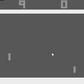
\includegraphics[scale=2.0]{figures/related_work/pong_729_pre_processed.jpeg}\par
    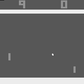
\includegraphics[scale=2.0]{figures/related_work/pong_729_pre_processed.png}\par
\end{multicols}
\caption{Pre-processed frames captured from Pong emulated on Stella. These frames were originally $84\times 84$, but are printed here as $168\times 168$ to emphasise distortions. \textbf{Left:} The JPEG format distorts the ball, paddle and score sprites. \textbf{Right:} The PNG format displays the frame without such distortions.}
\label{fig:pong_729_pre_processed}
\end{figure}


%
%
%
%
%
\section{Qualitative Assessment Using GUIs}


%
%
%
%
%
\section{Latent Image}
\lipsum[2]
\subsection{Architecture}
\begin{figure}[H]
\centering
\captionsetup{justification=centering}
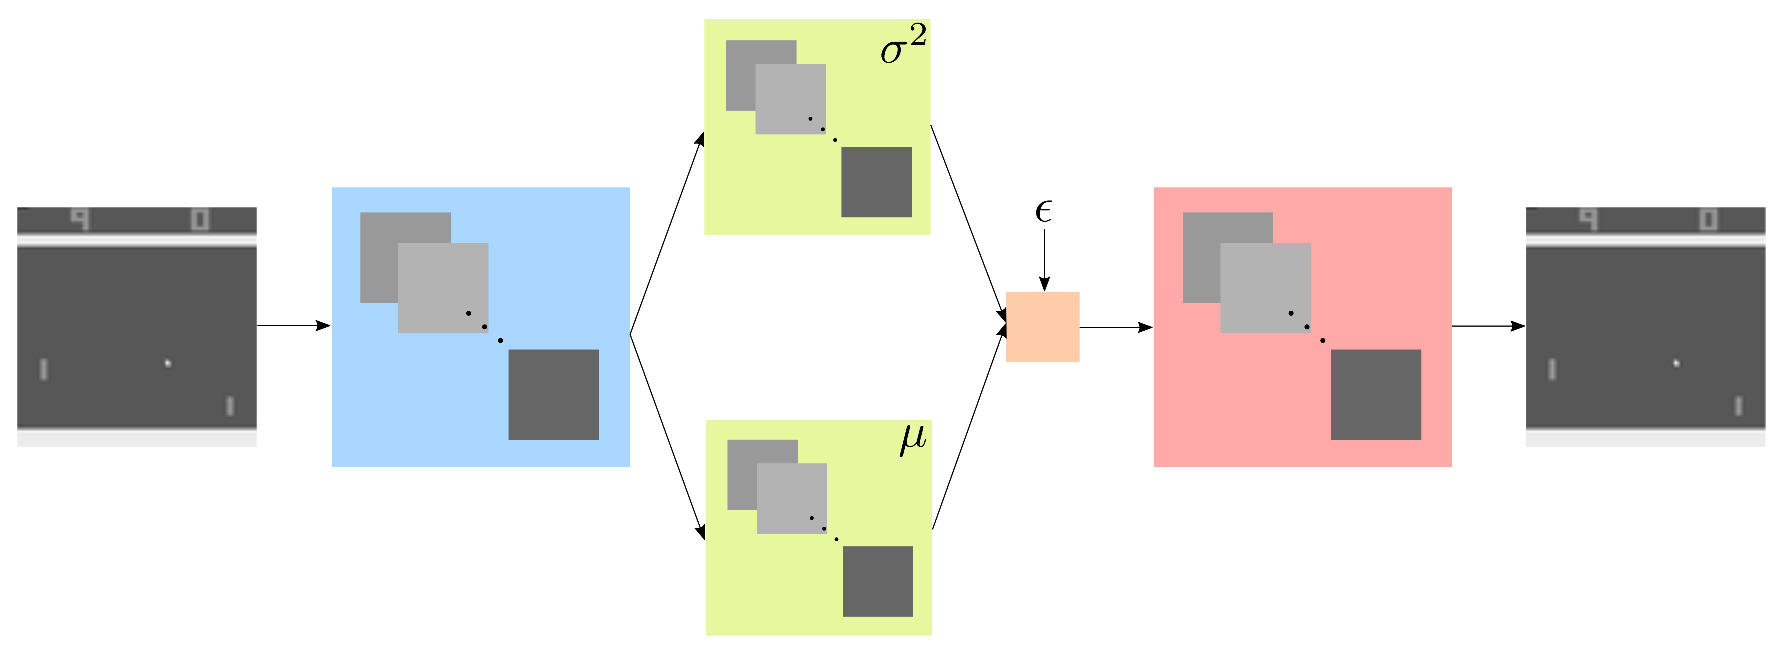
\includegraphics[scale=0.58]{methods/latent_image_architecture.eps}
\caption{Caption.}
\label{fig:latent_image_architecture}
\end{figure}

\subsection{Derivation}

%
%
%
%
%
\section{Disentangling Latent Neurons}
\lipsum[2]
\subsection{Architecture}
\begin{figure}[H]
\centering
\captionsetup{justification=centering}
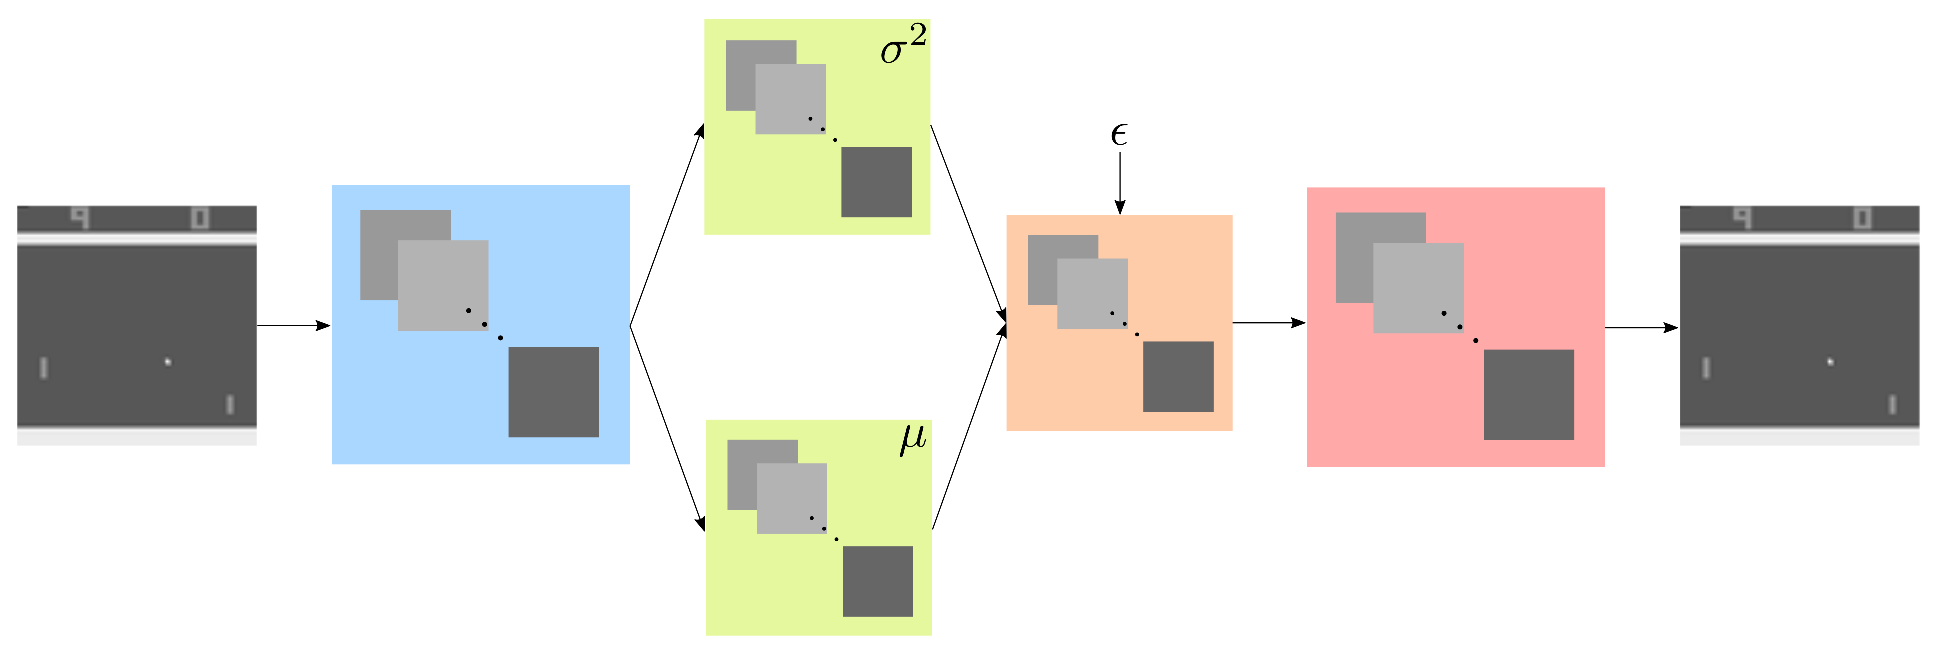
\includegraphics[scale=0.55]{methods/decoupling_indiscriminately_horizontal.eps}
\caption{Caption.}
\label{fig:decoupling_indiscriminately_horizontal}
\end{figure}

\begin{figure}[H]
\centering
\captionsetup{justification=centering}
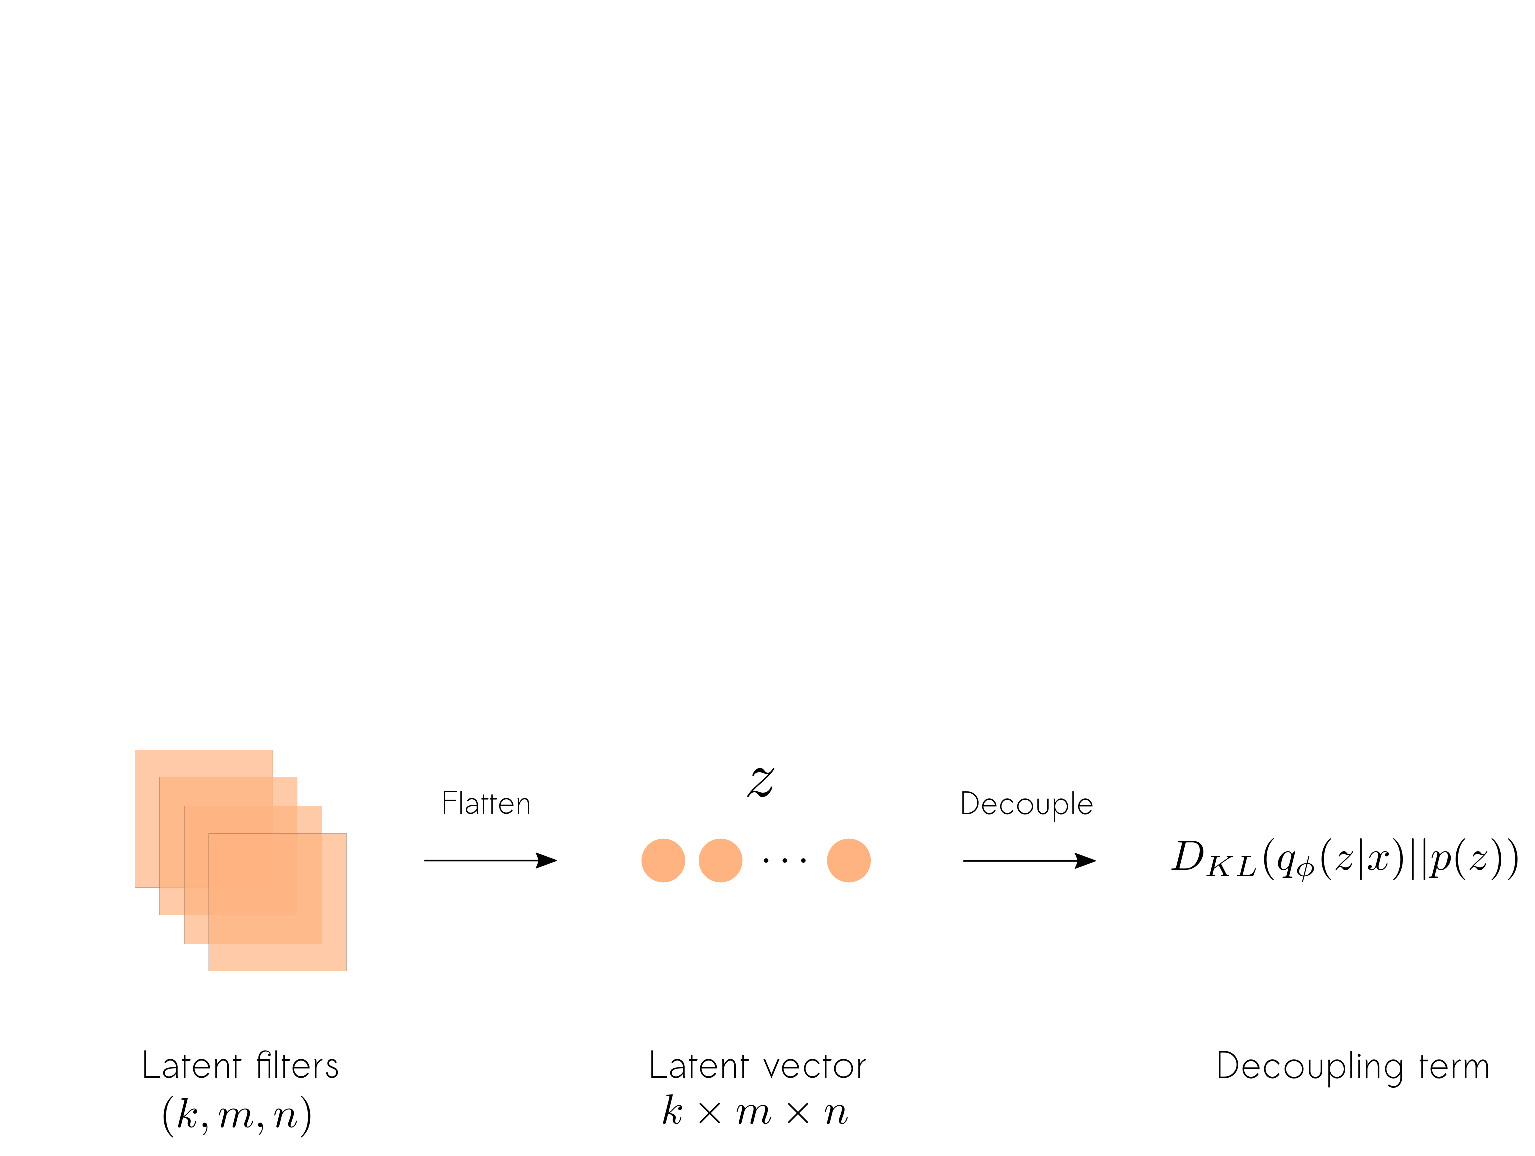
\includegraphics[scale=0.6]{methods/decoupling_indiscriminately_flattening_latent_space.eps}
\caption{Caption.}
\label{fig:decoupling_indiscriminately_flattening_latent_space}
\end{figure}

\subsection{Derivation}



%
%
%
%
%
\section{Disentangling Latent Filters Using Averages}
\lipsum[2]
\subsection{Architecture}
\begin{figure}[H]
\centering
\captionsetup{justification=centering}
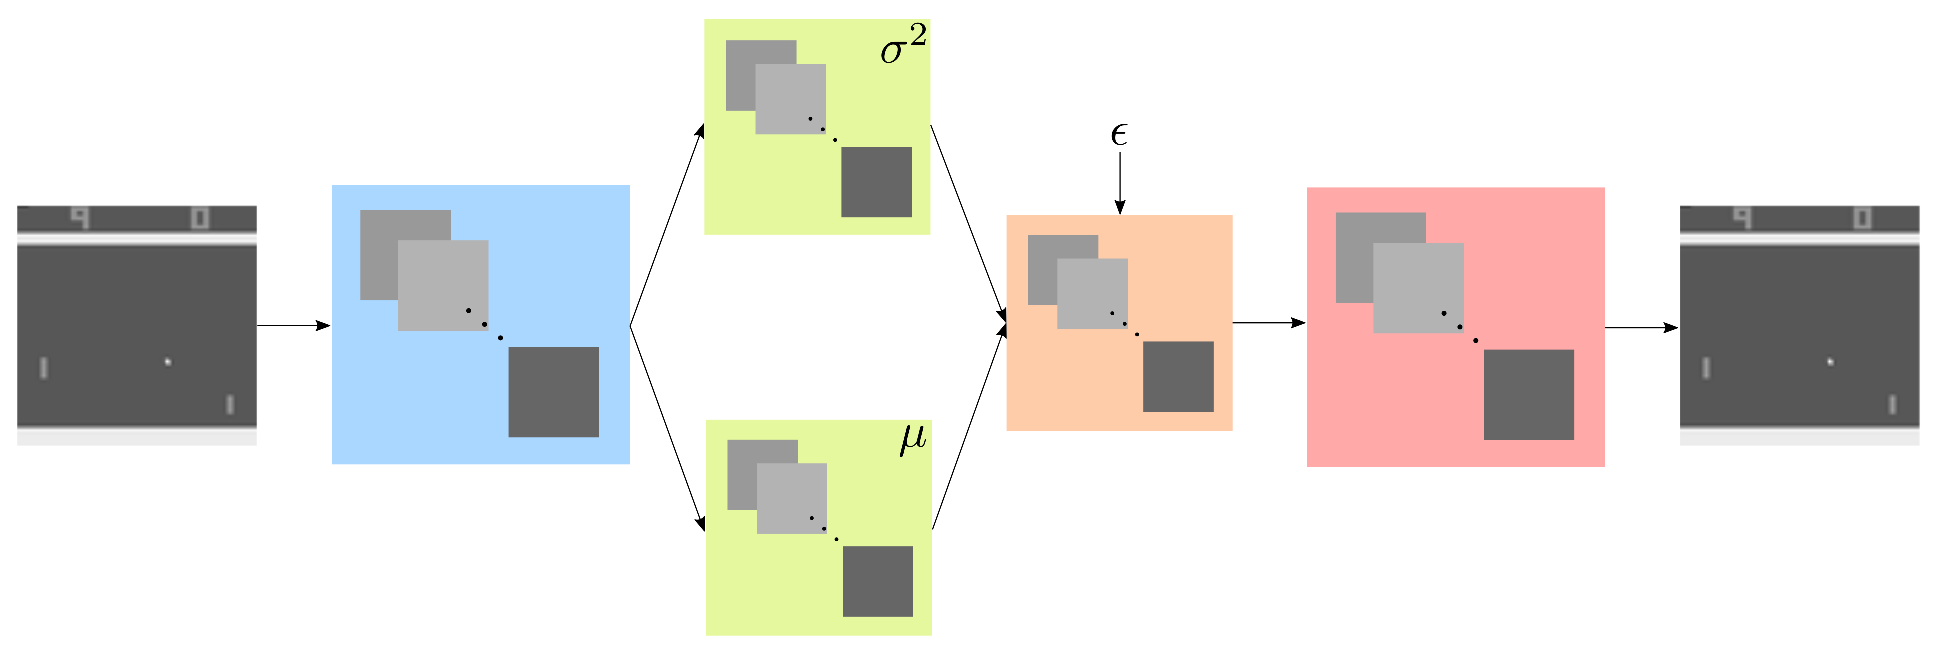
\includegraphics[scale=0.55]{methods/decoupling_indiscriminately_horizontal.eps}
\caption{Caption.}
\label{fig:decoupling_indiscriminately_horizontal}
\end{figure}

\begin{figure}[H]
\centering
\captionsetup{justification=centering}
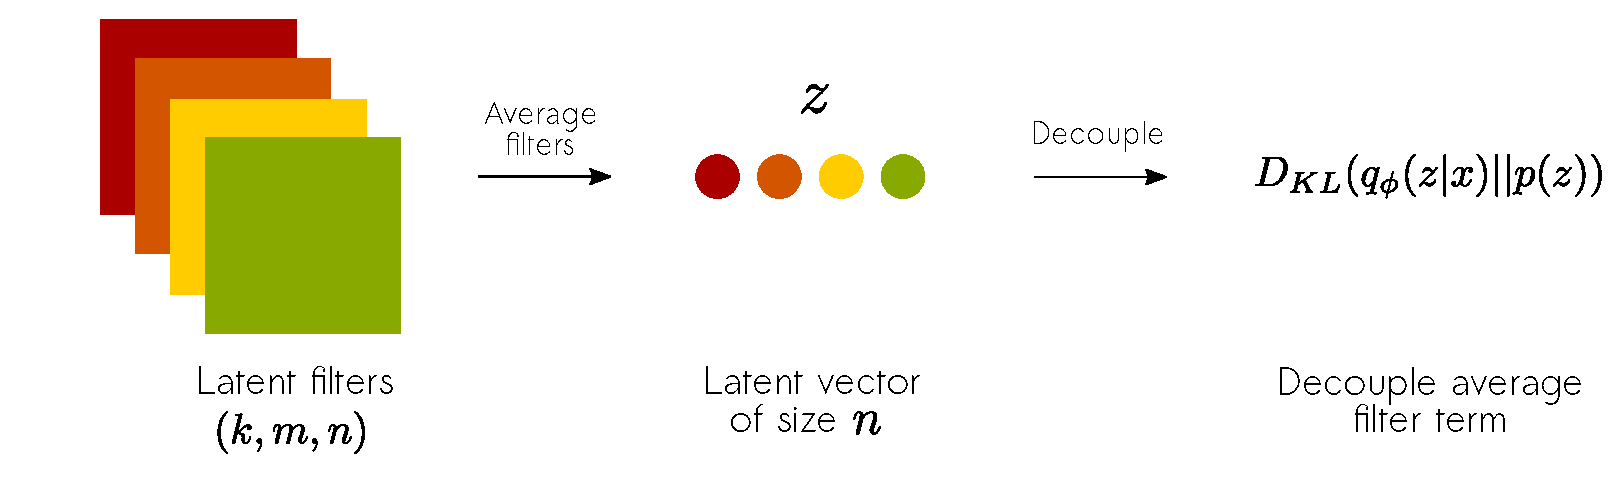
\includegraphics[scale=0.6]{methods/decoupling_averages_latent_space.eps}
\caption{Caption.}
\label{fig:decoupling_averages_latent_space}
\end{figure}

\subsection{Derivation}

%
%
%
%
%
\section{Decoupling Latent Filters Using Weighted-Averages}
\lipsum[2]
\subsection{Architecture}
\subsection{Derivation}

%
%
%
%
%
\section{Separating Colour Spaces}
\lipsum[2]
\subsection{Architecture}
\subsection{Derivation}

%
%
%
%
%
\section{Orthogonal Convolutions}
\lipsum[2]
\subsection{Architecture}
\begin{figure}[h!]
\centering
\captionsetup{justification=centering}
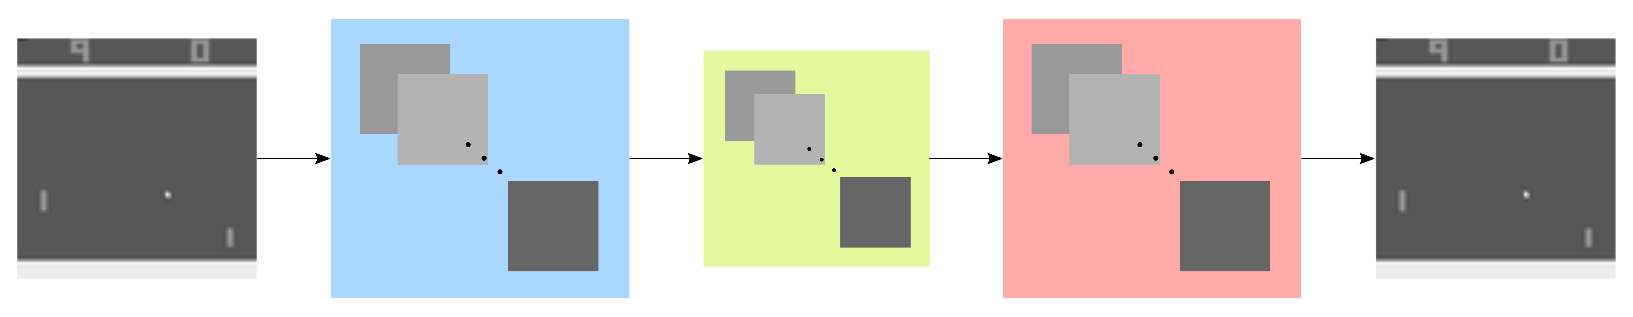
\includegraphics[scale=0.63]{methods/orthogonal_convolutions_archiecture.eps}
\caption{Caption.}
\label{fig:orthogonal_convolutions_archiecture}
\end{figure}

\subsection{Derivation}

%
%
%
%
%
\section{Winner Takes All}
\lipsum[2]
\subsection{Architecture}
\subsection{Derivation}
